The fixed synthetic dataset was evaluated across 3 held-out families and 5 seeds (15 runs), with up to 20 autoencoder epochs and 100 DQN episodes per run. Table~\ref{tab:recall} reports means and sample standard deviations, not confidence intervals.
\begin{table}[ht]\centering\caption{Synthetic held-out recall (five seeds).}\label{tab:recall}
\begin{tabular}{lcc}\toprule Family & Frozen DQN & RF mean \\ \midrule
Exploits & 1.000 $\pm$ 0.000 & 1.000 \\
Fuzzers & 0.947 $\pm$ 0.016 & 0.989 \\
Reconnaissance & 0.480 $\pm$ 0.094 & 0.487 \\
\bottomrule\end{tabular}\end{table}
\begin{figure}[ht]\centering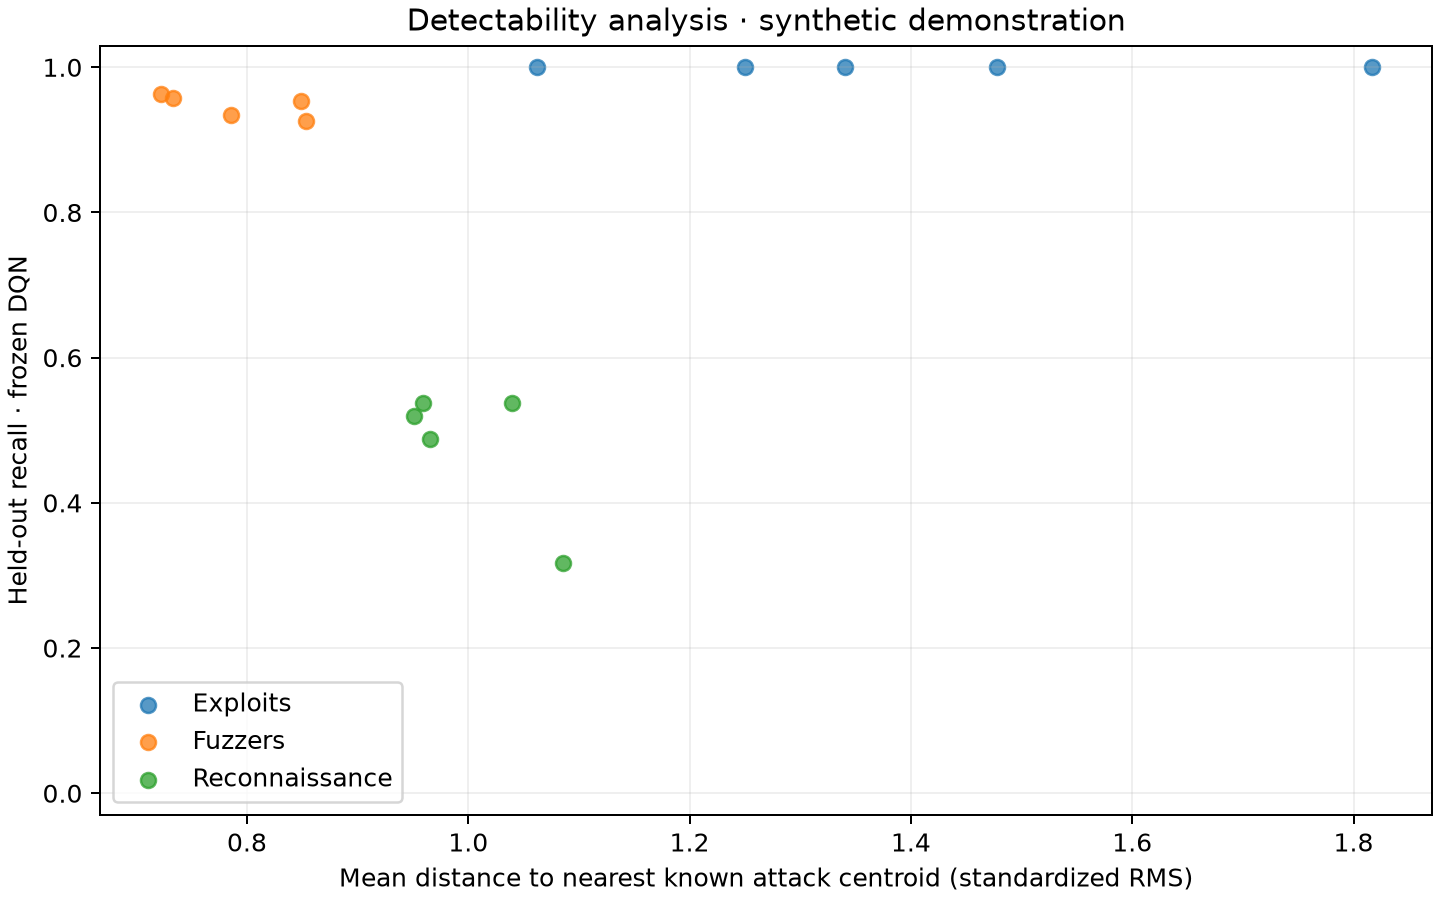
\includegraphics[width=\columnwidth]{detectability.png}\caption{Frozen DQN detectability on synthetic data. Each point is one held-out-family/seed run.}\end{figure}
These results characterize this synthetic generator only. Cross-family distance comparisons are exploratory because each encoder is trained separately.
Reconnaissance had mean distance 1.000 and recall 0.480, compared with Fuzzers
distance 0.789 and recall 0.947. Thus mean centroid distance did not monotonically
order detection performance in this experiment. Random Forest did not perform
worse than the frozen DQN on mean held-out recall for these three families.
On the local Intel CPU, ONNX Runtime 1.24.4 with one thread gave median batch
latencies of 0.0937, 0.2265 and 1.1846 ms at batch sizes 1, 32 and 256.
These are reconstruction-only measurements, not end-to-end detection latency.
